% !TEX TS-program = pdflatex
% !TEX encoding = UTF-8 Unicode

% This is a simple template for a LaTeX document using the "article" class.
% See "book", "report", "letter" for other types of document.

\documentclass[11pt]{article} % use larger type; default would be 10pt

\usepackage[utf8]{inputenc} % set input encoding (not needed with XeLaTeX)

%%% Examples of Article customizations
% These packages are optional, depending whether you want the features they provide.
% See the LaTeX Companion or other references for full information.
\usepackage{graphicx,parskip,appendix,float}
\usepackage[ruled]{algorithm2e}
\usepackage{url,amsmath,amssymb,fancybox,listings,pdfpages,caption,multicol,datetime,rotating, booktabs}
\usepackage{etoolbox}
%\usepackage[usenames,dvipsnames]{color} % Don't use it as it clashes with csquote
\usepackage{csquotes}
% \usepackage{subfig}
%\usepackage[T1]{fontenc}
\usepackage{enumerate}
\usepackage{tabularx}
\usepackage{derivative}
\usepackage{mathtools}
%\usepackage{enumitem}
%%% PAGE DIMENSIONS
\usepackage{geometry} % to change the page dimensions
\geometry{a4paper} % or letterpaper (US) or a5paper or....
 \geometry{margin=1in} % for example, change the margins to 2 inches all round
% \geometry{landscape} % set up the page for landscape
%   read geometry.pdf for detailed page layout information
\usepackage{hyperref}
\hypersetup{
    colorlinks=true,
    linkcolor=blue,
    filecolor=blue,      
    urlcolor=blue,
    citecolor=blue,
    pdftitle={Overleaf Example},
    pdfpagemode=FullScreen,
    }
\usepackage{graphicx} % support the \includegraphics command and options
\usepackage{subcaption}
\captionsetup{compatibility=false}
% \usepackage[parfill]{parskip} % Activate to begin paragraphs with an empty line rather than an indent

%%% PACKAGES
\usepackage{booktabs} % for much better looking tables
\usepackage{array} % for better arrays (eg matrices) in maths
\usepackage{paralist} % very flexible & customisable lists (eg. enumerate/itemize, etc.)
\usepackage{verbatim} % adds environment for commenting out blocks of text & for better verbatim
%\usepackage{subfig} % make it possible to include more than one captioned figure/table in a single float
% These packages are all incorporated in the memoir class to one degree or another...
%\usepackage{listings}
%\usepackage{xcolor}

\definecolor{colBackGrnd}{rgb}{1,1,0.8}
\definecolor{colKeys}{rgb}{0,0,1}
\definecolor{colIdentifier}{rgb}{0,0,0}
\definecolor{colComments}{rgb}{0,.5,0}
\definecolor{colString}{rgb}{0,0,1}
\definecolor{colWhite}{rgb}{1,1,1}

\lstset{%
    float=H,
    basicstyle=\ttfamily\footnotesize,
    identifierstyle=\color{colIdentifier},
    keywordstyle=\color{colIdentifier}, %
    stringstyle=\color{colIdentifier},
    commentstyle=\color{colIdentifier}, %
    columns=flexible,
    tabsize=2,
    frame=single,
    extendedchars=true, %
    showspaces=false,
    showstringspaces=false,
    numbers=left, %
    numberstyle=\footnotesize,
    breaklines=true,
    language=Java,
    backgroundcolor=\color{colBackGrnd},
    breakautoindent=true, %
    captionpos=b%
}

%\lstset{style=mystyle}
%%% HEADERS & FOOTERS
\usepackage{fancyhdr} % This should be set AFTER setting up the page geometry
\pagestyle{fancy} % options: empty , plain , fancy
\renewcommand{\headrulewidth}{0pt} % customise the layout...
\lhead{}\chead{}\rhead{}
\lfoot{}\cfoot{\thepage}\rfoot{}

%%% SECTION TITLE APPEARANCE
%\usepackage{sectsty}
%\allsectionsfont{\sffamily\mdseries\upshape} % (See the fntguide.pdf for font help)
% (This matches ConTeXt defaults)

%%% ToC (table of contents) APPEARANCE
\usepackage[nottoc,notlof,notlot]{tocbibind} % Put the bibliography in the ToC
\usepackage[titles,subfigure]{tocloft} % Alter the style of the Table of Contents
\renewcommand{\cftsecfont}{\rmfamily\mdseries\upshape}
\renewcommand{\cftsecpagefont}{\rmfamily\mdseries\upshape} % No bold!
\usepackage{underscore}
%%% END Article customizations

\begin{document}
    \begin{titlepage}
    \centering
    \vspace*{\fill}
    \LARGE{\textbf{MTH 602 Scientific Machine Learning}}\\
    \vspace*{0.3cm}
    \Large{Homework 1}\\
     \vspace*{0.3cm}
    9/22/2025\\
         \vspace*{2cm}
   S. M. Mahfuzul Hasan\\
        \vspace*{0.3cm}
   02181922\\
        \vspace*{2.5cm}
   
\includegraphics[width=6cm]{umassd-standard-2color-logo-LG-1}
    \vspace*{\fill}
    \end{titlepage}


\begin{enumerate}
\renewcommand{\labelenumi}{\bfseries\theenumi.}
\item Given, 
\begin{equation*}
\phi(x_1, x_2, x_3) = \frac{1}{\sqrt{x_1^2+x_2^2+x_3^2}}
\end{equation*}
\begin{enumerate}[\textbf{(\alph*)}]
\renewcommand{\labelenumi}{\bfseries\theenumi.}
\item
\begin{equation*}
\begin{split}
\Vec F = \nabla\phi &= \left(\frac{\partial}{\partial {x_1}}\hat i + \frac{\partial}{\partial {x_2}}\hat j + \frac{\partial}{\partial {x_3}}\hat k\right)\frac{1}{\sqrt{x_1^2+x_2^2+x_3^2}}\\
&=\frac{-1}{2\sqrt{{\left(x_1^2+x_2^2+x_3^2\right)}^3}}\left(2x_1\hat i  + 2x_2\hat j  + 2x_3\hat k \right)\\
&=\frac{-1}{\sqrt{{\left(x_1^2+x_2^2+x_3^2\right)}^3}}\left(x_1\hat i  + x_2\hat j  + x_3\hat k \right) \hspace{0.5cm} \text{(Ans.)}
\end{split}
\end{equation*}
\item
At (1, 0, 0),
\begin{equation*}
\begin{split}
\Vec F (1, 0, 0) &=\frac{-1}{\sqrt{{\left(1^2+0^2+0^2\right)}^3}}\left(1\hat i  + 0\hat j  + 0\hat k \right) \\
&= -\hat i \hspace{0.5cm} \text{(Ans.)}
\end{split}
\end{equation*}
\begin{tabular}{ll}
Direction: &along (-)ve $x_1$ axis. \\
Magnitude:  &${\| \Vec F (1, 0, 0) \|}_2^2 = \sqrt{{\left(-1\right)}^2} = 1$
\end{tabular}
\begin{figure}[!htb]
    \centering
        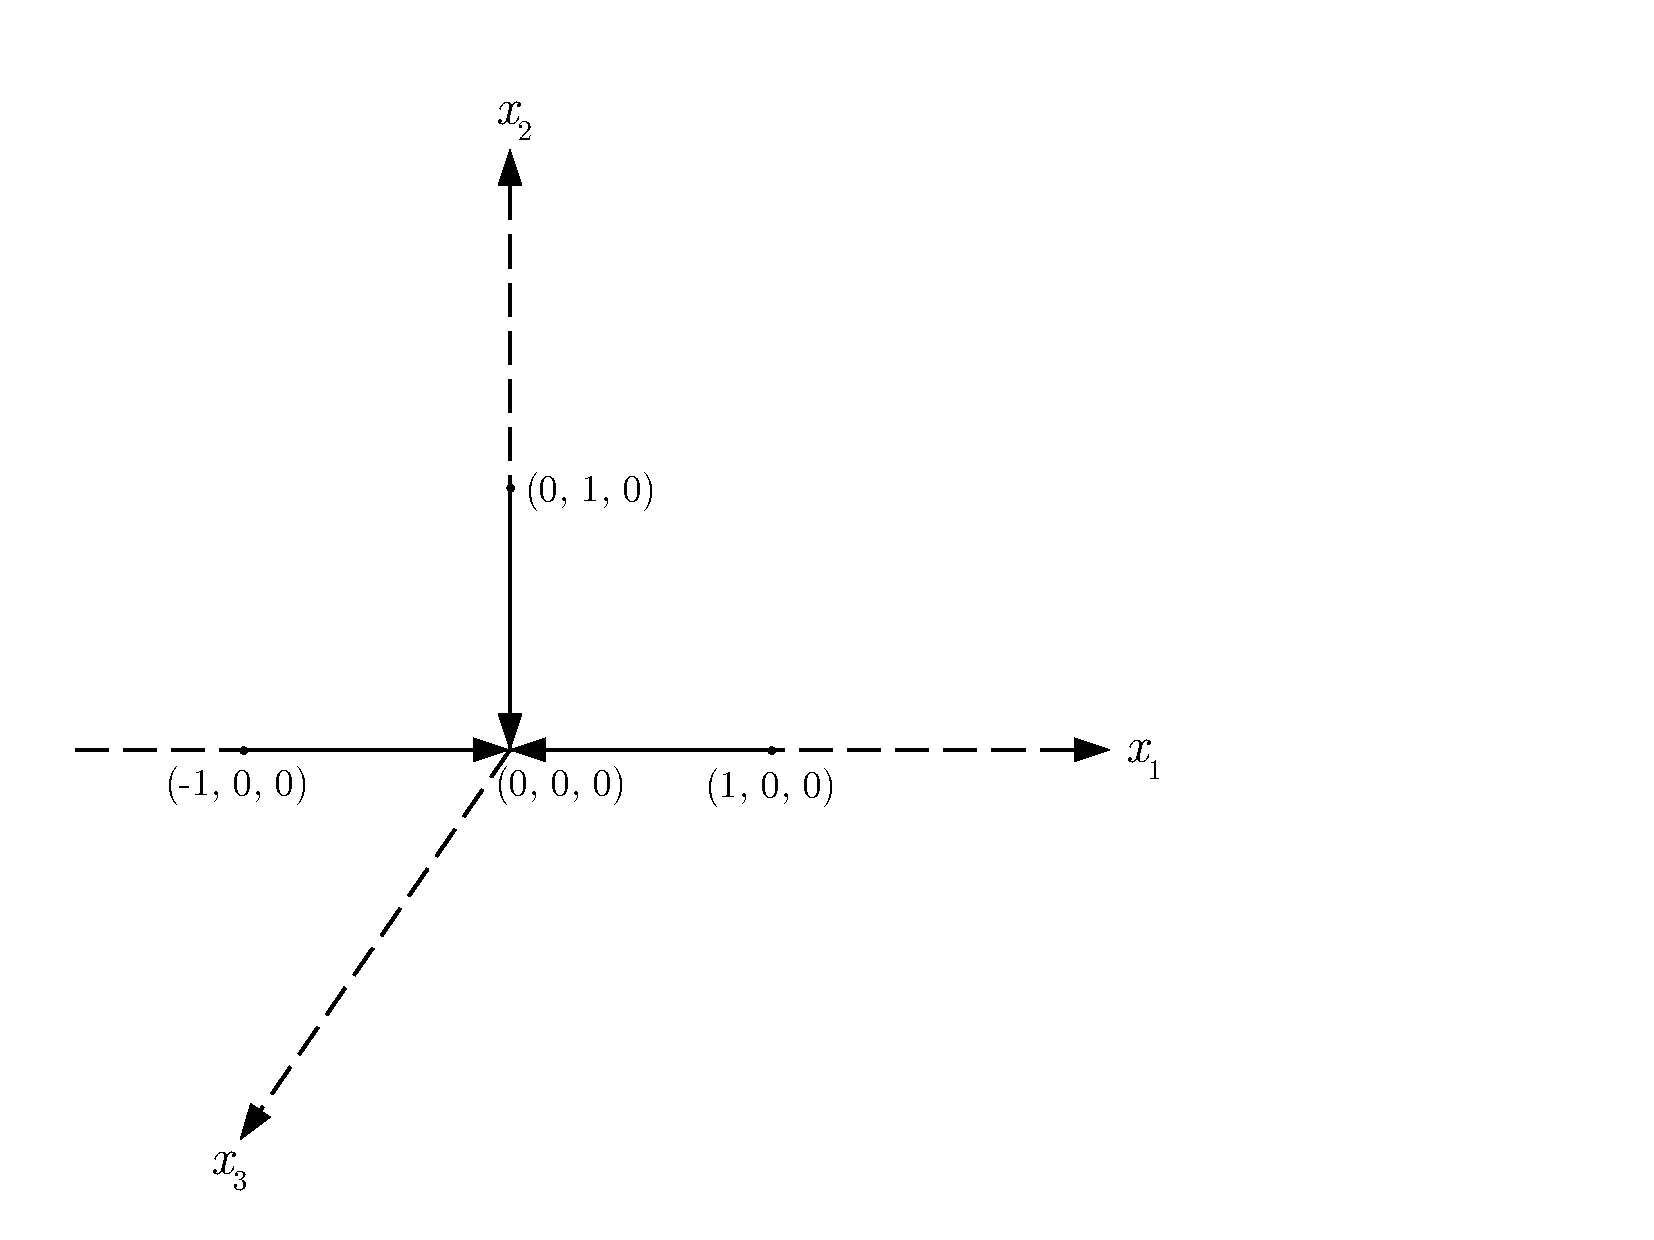
\includegraphics[width=10cm,trim={1cm 0cm 8cm 1cm},clip]{vector}
    \caption{Sketch of $\Vec F$ at (1, 0, 0), (-1, 0, 0) and (0, 1, 0).}
    \label{fig1}
\end{figure}

At (-1, 0, 0),
\begin{equation*}
\begin{split}
\Vec F (-1, 0, 0) &=\frac{-1}{\sqrt{{\left({\left(-1\right)}^2+0^2+0^2\right)}^3}}\left(-1\hat i  + 0\hat j  + 0\hat k \right) \\
&= \hat i \hspace{0.5cm} \text{(Ans.)}
\end{split}
\end{equation*}
\begin{tabular}{ll}
Direction: &along (+)ve $x_1$ axis. \\
Magnitude:  &${\| \Vec F (-1, 0, 0) \|}_2^2 = \sqrt{1^2} = 1$
\end{tabular}

At (0, 1, 0),
\begin{equation*}
\begin{split}
\Vec F (0, 1, 0) &=\frac{-1}{\sqrt{{\left(0^2+1^2+0^2\right)}^3}}\left(0\hat i  + 1\hat j  + 0\hat k \right) \\
&= -\hat j \hspace{0.5cm} \text{(Ans.)}
\end{split}
\end{equation*}
\begin{tabular}{ll}
Direction: &along (-)ve $x_2$ axis. \\
Magnitude:  &${\| \Vec F (0, 1, 0) \|}_2^2 = \sqrt{{\left(1\right)}^2} = 1$
\end{tabular}
\end{enumerate}

\item Given,
\begin{equation*}
\begin{split}
&\left<\Vec x,\Vec y\right> = {\Vec x}^T\Vec y, \hspace{0.2cm}\text{where}\hspace{0.1cm} \Vec x,\Vec y \in \mathbb{R}^{N}\\
&Q^TQ = I, \hspace{0.2cm}\text{where}\hspace{0.1cm} Q \in \mathbb{R}^{N\times N}
\end{split}
\end{equation*}
\begin{enumerate}[\textbf{(\alph*)}]
\renewcommand{\labelenumi}{\bfseries\theenumi.}
\item
\begin{equation*}
\begin{split}
\text{L.H.S} = &\left<Q\Vec x, Q\Vec y\right> = {\left(Q\Vec x\right)}^T\left(Q\Vec y\right) = \left({\Vec x}^TQ^T\right)\left(Q\Vec y\right) = {\Vec x}^T\left(Q^TQ\right)\Vec y \\
&= {\Vec x}^TI\Vec y = {\Vec x}^T\Vec y = \left<\Vec x,\Vec y\right> = \text{R.H.S} \hspace{0.5cm} \text{(Showed)}
\end{split}
\end{equation*}
\item
\begin{equation*}
\begin{split}
\|Q\Vec x\|_2 &= \sqrt{{\left(Q\Vec x\right)}^T\left(Q\Vec x\right)} = \sqrt{\left({\Vec x}^TQ^T\right)\left(Q\Vec x\right)} = \sqrt{{\Vec x}^T\left(Q^TQ\right)\Vec x} \\
&= \sqrt{{\Vec x}^TI\Vec x} = \sqrt{{\Vec x}^T\Vec x} = \|\Vec x\|_2
\end{split}
\end{equation*}
\end{enumerate}

\item
To verify,
\begin{equation*}
\begin{split}
&\|\Vec x\|_{\infty} \leq \|\Vec x\|_{2} \\
&\|\Vec x\|_2 \leq \sqrt{N}\|\Vec x\|_{\infty} 
\end{split}
\end{equation*}
\begin{enumerate}[\textbf{(\alph*)}]
\renewcommand{\labelenumi}{\bfseries\theenumi.}
\item 
\begin{equation}
\begin{split}
&\|\Vec x\|_{\infty} = \max\limits_{1\leq i \leq N}{\vert x_i\vert}
\end{split}
\label{eq1}
\end{equation}
Let's arrange the elements of $\Vec x$ in such a way that the maximum absolute valued element sits at $N^{th}$ position. Then equation (\ref{eq1}) becomes-
\begin{equation}
\begin{split}
&\|\Vec x\|_{\infty} = \vert x_N\vert
\end{split}
\label{eq2}
\end{equation}
Now,
\begin{equation*}
\begin{split}
&\|\Vec x\|_2 = \sqrt{\sum\limits_{i=1}^N{\vert x_i\vert}^2} = \sqrt{\sum\limits_{i=1}^{N-1}{\vert x_i\vert}^2+{\vert x_N\vert}^2}  \\
&\Rightarrow \|\Vec x\|_2 \geq \sqrt{{\vert x_N\vert}^2}, \hspace{0.5cm} \text{since, $\sum\limits_{i=1}^{N-1}{\vert x_i\vert}^2 \geq 0$}\\
&\Rightarrow \|\Vec x\|_2 \geq \sqrt{{(\|\Vec x\|_{\infty})}^2}, \hspace{0.5cm} \text{from equation (\ref{eq2})}\\
&\Rightarrow \|\Vec x\|_{\infty} \leq \|\Vec x\|_2 \hspace{0.5cm} \text{(Verified)}
\end{split}
\end{equation*}

\item We know,
\begin{equation}
\begin{split}
&\vert x_i \vert \leq \max\limits_{1\leq i \leq N} \vert x_i\vert, \hspace{0.5cm} \text{for any $i \in [1, N]$}
\end{split}
\label{eq3}
\end{equation}
Let's assume again that the maximum absolute valued element is $x_N$. Then equation (\ref{eq3}) can be written as,
\begin{equation*}
\begin{split}
&{\vert x_i \vert}^2 \leq {\vert x_N\vert}^2\\
&\Rightarrow \sum\limits_{i=1}^N {\vert x_i \vert}^2 \leq \sum\limits_{i=1}^N {\vert x_N\vert}^2 = N{\vert x_N\vert}^2\\
&\Rightarrow \sqrt{\sum\limits_{i=1}^N{\vert x_i\vert}^2} \leq \sqrt{N{\vert x_N\vert}^2}\\
&\Rightarrow \|\Vec x\|_2 \leq \sqrt{N}\|\Vec x\|_{\infty} \hspace{0.5cm} \text{(Verified)}
\end{split}
\end{equation*}
\end{enumerate}

\item
Let,
\[A \in \mathbb{R}^{N\times(M+1)}, \Vec y \in \mathbb{R}^{N}, \Vec \omega \in \mathbb{R}^{M+1}\]
\begin{enumerate}[\textbf{(\alph*)}]
\renewcommand{\labelenumi}{\bfseries\theenumi.}
\item 
\begin{equation*}
\begin{split}
\|\Vec y - A\Vec \omega\|_2^2 &= {\left(\Vec y - A\Vec \omega\right)}^T\left(\Vec y - A\Vec \omega\right)\\
&= \left({\Vec y}^T - {\left(A\Vec \omega\right)}^T\right)\left(\Vec y - A\Vec \omega\right), \hspace{0.5cm} \text{since, ${(X-Y)}^T = X^T - Y^T$}\\
&=\Vec y^T \Vec y - \Vec y^T(A\Vec \omega) - {(A\Vec \omega)}^T\Vec y + {(A\Vec \omega)}^T(A\Vec \omega)\\
&= \Vec y^T \Vec y - {\left(\Vec y^T(A\Vec \omega)\right)}^T - {(A\Vec \omega)}^T\Vec y + {(A\Vec \omega)}^T(A\Vec \omega),\\
&\hspace{5.25cm} \text{since, $\Vec y^T(A\Vec \omega)$ is a scalar quantity}\\
&= \Vec y^T \Vec y - {(A\Vec \omega)}^T{\left(\Vec y^T\right)}^T - {(A\Vec \omega)}^T\Vec y + {(A\Vec \omega)}^T(A\Vec \omega), \\
&\hspace{5.25cm} \text{since, ${(XY)}^T = Y^TX^T$}\\
&= \Vec y^T \Vec y - {(A\Vec \omega)}^T\Vec y - {(A\Vec \omega)}^T\Vec y + {(A\Vec \omega)}^T(A\Vec \omega), \\
&\hspace{5.25cm} \text{since, ${\left(X^T\right)}^T = X$}\\
&= \Vec y^T \Vec y - 2{(A\Vec \omega)}^T\Vec y+ {(A\Vec \omega)}^T(A\Vec \omega) \\
&= {\Vec \omega}^TA^TA\Vec \omega - 2{\Vec \omega}^TA^T \Vec y  + \Vec y^T \Vec y  \hspace{0.5cm} \text{(Showed)}
\end{split}
\end{equation*}
Note: $X$ and $Y$ are representative matrices.

\item 
\begin{equation}
\begin{split}
\nabla_{\Vec{\omega}}\|\Vec y - A\Vec \omega\|_2^2 &= \nabla_{\Vec{\omega}}\left({\Vec \omega}^TA^TA\Vec \omega - 2{\Vec \omega}^TA^T \Vec y  + \Vec y^T \Vec y \right)
\end{split}
\label{eq4}
\end{equation}
\begin{equation*}
\begin{split}
\nabla_{\Vec{\omega}}\left({\Vec \omega}^TA^TA\Vec \omega\right) &= (A^TA+{\left(A^TA\right)}^T)\Vec \omega, \\
&\hspace{1cm} \text{using $\nabla_{\Vec{\omega}}\left({\Vec \omega}^TB\Vec \omega\right) = (B+B^T)\Vec \omega$, where $B=A^TA$ here}\\
&=\left(A^TA+A^TA\right)\Vec \omega = 2A^TA\Vec \omega
\end{split}
\end{equation*}
\begin{equation*}
\begin{split}
\nabla_{\Vec{\omega}}\left({\Vec \omega}^TA^T\Vec y\right) &= A^T\Vec y, \\
&\hspace{1cm} \text{using $\nabla_{\Vec{\omega}}\left({\Vec \omega}^T\Vec {y'}\right) = \Vec {y'}$, where $\Vec {y'}=A^T\Vec y$ here}
\end{split}
\end{equation*}
\begin{equation*}
\begin{split}
\nabla_{\Vec{\omega}}\left({\Vec y}^T\Vec y\right) &= 0, \hspace{0.5cm} \text{since, $\Vec y$ does not depend on $\Vec \omega$}
\end{split}
\end{equation*}
So, equation (\ref{eq4}) becomes-
\begin{equation}
\begin{split}
\nabla_{\Vec{\omega}}\|\Vec y - A\Vec \omega\|_2^2 &= 2A^TA\Vec \omega - 2A^T\Vec y + 0 = 2A^TA\Vec \omega - 2A^T\Vec y \hspace{0.5cm}\text{(Showed)}
\end{split}
\label{eq5}
\end{equation}
\end{enumerate}
\item Projection matrix is defined as,
\[P = A\left(A^TA\right)^{-1}A^T\]
\begin{enumerate}[\textbf{(\alph*)}]
\renewcommand{\labelenumi}{\bfseries\theenumi.}
\item 
\begin{equation*}
\begin{split}
L.H.S = P(P\Vec y) &= A\left(A^TA\right)^{-1}A^T\left(A\left(A^TA\right)^{-1}A^T \Vec y\right)\\
&= A\left(\left(A^TA\right)^{-1}A^TA\right)\left(A^TA\right)^{-1}A^T \Vec y\\
&=AI\left(A^TA\right)^{-1}A^T \Vec y, \\
&\hspace{1cm} \text{since, $A^TA$ is a square matrix $\left(\in \mathbb R^{(M+1)\times(M+1)}\right)$ and invertible}\\
&= A\left(A^TA\right)^{-1}A^T \Vec y = P\Vec y = R.H.S \hspace{0.5cm} \text{(Showed)}
\end{split}
\end{equation*}

\item 
\begin{equation*}
\begin{split}
L.H.S = P\Vec y_M &= A\left(A^TA\right)^{-1}A^T \Vec y_M \\
&= A\left(A^TA\right)^{-1}A^T(A\Vec \omega)\\
&= A\left(\left(A^TA\right)^{-1}A^TA\right)\Vec \omega \\
&= AI\Vec \omega = A\Vec \omega = \Vec y_M = R.H.S \hspace{0.5cm} \text{(Showed)}
\end{split}
\end{equation*}

\item The condition for least squares solution as derived in equation (\ref{eq5}) is
\begin{equation}
\begin{split}
\nabla_{\Vec{\omega}}\|\Vec r\|_2^2 = \nabla_{\Vec{\omega}}\|\Vec y - \Vec y_M\|_2^2 &= 2A^TA\Vec \omega_* - 2A^T\Vec y = 0 \\
&\Rightarrow A^TA\Vec \omega_* - A^T\Vec y = 0
\end{split}
\label{eq6}
\end{equation}
Now, 
\begin{equation*}
\begin{split}
L.H.S = P\vec r &= A\left(A^TA\right)^{-1}A^T\left(\Vec y - \Vec y_M\right) \\
&= A\left(A^TA\right)^{-1}\left(A^T\Vec y - A^T\Vec y_M\right)\\
&= A\left(A^TA\right)^{-1}\left(A^T\Vec y - A^TA\Vec\omega_*\right), \hspace{0.5cm} \text{since, $\Vec y_M = A\Vec\omega_*$}\\
&= A\left(A^TA\right)^{-1} (0), \hspace{0.5cm} \text{from equation (\ref{eq6})}\\
&= 0 =R.H.S \hspace{0.5cm} \text{(Showed)}
\end{split}
\end{equation*}
\end{enumerate}
\end{enumerate}
\iffalse
Fixed point is a point of a function that outputs itself when it is inputted into a function. Let $p$ be a point in the \textit{domain} of the function $g(x)$ such that, $g(p) = p$. Here, $p$ exists in the both \textit{domain}, and \textit{range} of the function $g(x)$, unchanged by the transformation.
\begin{figure}[!htb]
    \centering
    \begin{subfigure}{.5\textwidth}
        \centering
        \includegraphics[width=10cm,trim={5cm 8.5cm 3cm 9cm},clip]{fxd1}
        \caption{$g_1(x) = x - x^5$}
        \label{fig1a}
    \end{subfigure}\hfill
    \begin{subfigure}{0.5\textwidth}
        \centering
        \includegraphics[width=10cm,trim={5cm 8.5cm 3cm 9cm},clip]{fxd2}
        \caption{$g_2(x) = x + x^5$}
        \label{fig1b}
    \end{subfigure}
    \caption{Examples of fixed point using the given functions.}
    \label{fig1}
\end{figure}
As example, the fixed point of the two given functions will be such that we can write them as,
\begin{equation}
\centering
g_1(x) = x - x^5 = x
\label{eq1}
\end{equation}
\begin{equation}
\centering
g_2(x) = x + x^5 = x
\label{eq2}
\end{equation}
The fixed points for these two functions can be found by locating the intersection point of these two functions with $y = x$ line, which has been shown in figure \ref{fig1}. In both the cases, $x = 0$ is the fixed point, as that is the intersection point of $g_1(x)$, and $g_2(x)$ with $y = x$. It can be further proved by showing,
\begin{equation}
\centering
g_1(0) = 0 - 0^5 = 0,  \hspace{0.5cm} g_2(0) = 0 + 0^5 = 0,
\label{eq3}
\end{equation}
which is consistent with the definition of the fixed point as stated earlier.

\textbf{Q2: How is the fixed-point iteration applied to move from the current iteration \textbf{$p_n$} to the
next iteration \textbf{$p_{n+1}$}? Provide the formula used in this iteration process.}

For the fixed point iteration, the output of the function $g(x)$ at the first iteration step is taken as the input for the second iteration step. For a fixed point $x$ in function $g(x)$, it can be written as,
\begin{equation}
\centering
x_{n+1} = g(x_n); \hspace{0.5cm} n\geq0
\label{eq4}
\end{equation}
For the given functions, if the solution at current iteration is $p_n$, the formulae for advancing the solution to next iteration are,
\begin{equation}
\centering
p_{n+1} = g_1(p_n) = p_n - p_n^5
\label{eq5}
\end{equation}
\begin{equation}
\centering
p_{n+1} = g_1(p_n) = p_n + p_n^5
\label{eq6}
\end{equation}
\textbf{Q3+Q4: Does the fixed-point iteration provide a good approximation of the fixed point? Observe and discuss the convergence speed of the iteration.}

For the pursuit of obtaining the fixed point using fixed point iteration, we need to look into two theorems that give an indication of-
\begin{enumerate}[i.]
\item whether the convergence is possible.
\item which initial value(s) is (are) good enough in a region of search to find the fixed point using fixed point iteration.
\end{enumerate}

\textbf{Theorem-1:}\\
 If a function $g$ is continuous in [a, b], and $g(x) \in [a, b]$ for all $x \in [a, b]$, then there must be at least one fixed point in [a, b].
 
\textbf{Theorem-2:}\\
 If, in addition, $g'(x)$ exists in (a, b) such that, 
\begin{equation}
\centering
\left |g'(x)\right| \leq k, \hspace{0.5cm} \text{for all $x \in (a, b)$},
\label{eq7}
\end{equation}
where $k < 1$, then there is exactly one (unique) fixed point in [a, b].

\begin{figure}[!htb]
    \centering
        \includegraphics[width=10cm,trim={5cm 8.5cm 5cm 9cm},clip]{f1}
    \caption{Check for \textit{existence} and \textit{uniqueness}.}
    \label{fig2}
\end{figure}
\textbf{Fixed point iteration of \textbf{$g_1(x) = x - x^5$}}\\
First the \textit{existence} condition is checked using \textit{Theorem}-1. The function $g_1(x)$ is continuous in [-1, 1] because for $x \in [-1, 1]$, there exists $g_1(x) \in [-1, 1]$. Hence, it is concluded that there is at least one fixed point for this function in [-1, 1]. One thing to notice is that the same can be applied to other bound existing within [-1, 1] (for example, [-0.5, 0.5]).

Now, from figure \ref{fig2}, it is evident that though the function satisfies the requirement of \textit{Theorem}-1, it does not satisfy the requirement of \textit{Theorem}-2. It can be seen that the first derivative of $\left|g_1(x)\right|$ equals to 1 at $x = 0$ (which is the fixed point of the function), and is greater than 1 for some values of $x$ close to $x = -1, \text{or}  1$. It can be understood analytically as well as shown below.
\begin{equation}
\begin{gathered}
g_1'(x) = 1 - 5x^4\\
\left|g_1'(0)\right| = \left|1 - 5\cdot 0^4\right| = 1 > k,\hspace{0.5cm}
\left|g_1'(0.8)\right| = \left|1 - 5\cdot 0.8^4\right| = 1.048 > k
\label{eq8}
\end{gathered}
\end{equation}
So, there does not exist a $g_1'(x)$ in (-1, 1) for all $x \in (-1, 1)$, for which it is always maintained that $\left|g_1'(x)\right| \leq k$, where $k < 1$. As a result, there is no unique (one) fixed point in (-1, 1).
\begin{figure}[!htb]
    \centering
    \begin{subfigure}{.5\textwidth}
        \centering
        \includegraphics[width=10cm,trim={5cm 8cm 3cm 9cm},clip]{g1_0.1}
        \caption{}
        \label{fig3a}
    \end{subfigure}\hfill
    \begin{subfigure}{0.5\textwidth}
        \centering
        \includegraphics[width=10cm,trim={5cm 8cm 3cm 9cm},clip]{g1_0.5}
        \caption{}
        \label{fig3b}
    \end{subfigure}
    \caption{Convergence history of fixed point for initial guess (a) $x_0 = 0.1$, and (b) $x_0 = 0.5$.}
    \label{fig3}
\end{figure}
However, there are some points in (-1, 1) that maintain that $\left|g_1'(x)\right| \leq k$. If any one of such points is taken as an initial guess, then the solution can converge towards the fixed point $x = 0$ asymptotically. And, it is found that the convergence is very slow, and it would take infinite number of iterations to reach the fixed point. Even with infinite number of iterations, it is almost impossible to get close to the absolute error of $\sim$0.01 with respect to the fixed point.
\begin{figure}[!htb]
    \centering
    \begin{subfigure}{.5\textwidth}
        \centering
        \includegraphics[width=10cm,trim={4.5cm 8cm 3cm 9cm},clip]{g2_0.1}
        \caption{}
        \label{fig4a}
    \end{subfigure}\hfill
    \begin{subfigure}{0.5\textwidth}
        \centering
        \includegraphics[width=10cm,trim={4.5cm 8cm 3cm 9cm},clip]{g2_0.5}
        \caption{}
        \label{fig4b}
    \end{subfigure}
    \caption{Absolute error history using consecutive iterates, and the fixed point (found using \texttt{fzero}) for initial guess (a) $x_0 = 0.1$, and (b) $x_0 = 0.5$.}
    \label{fig4}
\end{figure}
From figure \ref{fig3}, and \ref{fig4}, some observations are made based on two different initial guesses for which $\left|g_1'(x)\right| \leq k$ with maximum no. of iterations of $10^6$.
\begin{enumerate}
\item From figure \ref{fig3}, the updated iterates become very close to the function value from the very start, but they never become equal. As a result, for both $x_0 = 0.1$, and $x_0 = 0.5$, the iterates approach $\sim$0.02 asymptotically, which still remain far away from the analytically obtained fixed point $x = 0$.
\item Convergence behavior is insensitive to the initial guess, as it can be seen from figure \ref{fig3}, and \ref{fig4} that the convergence history, and the absolute error history are very similar. And, it is true for other initial guesses as well in (-1, 1), except for $x_0 = 0$.
\item While the absolute tolerance between two consecutive iterates becomes less than $10^{-8}$ (figure \ref{fig4}), the fixed point is still far away from the ${(10^6)}^{th}$ iterate as observed from absolute error with respect to fixed point $x_e$, obtained using \texttt{fzero} with the same initial guess. It shows that even a very small tolerance between two consecutive iterates does not guarantee the closeness of the solution to the fixed point.
\end{enumerate}

The same convergence behavior is observed for an initial guess $x_0 = 0.95$, for which $\left|g_1'(x)\right| > 1$ from figure \ref{fig5}. So, it can be concluded that no matter the value of $\left|g_1'(x)\right|$ in (-1, 1), it will always move towards the fixed point asymptotically with a bad final approximation. The asymptotic convergence behavior reflects the fact that with every iteration, the ratio of absolute error for two consecutive iterates approaches $\lambda = 1$, which is bad for good fixed point approximation.
\begin{equation}
\begin{split}
&\frac{\left|x_{n+1} - x_e\right|}{\left|x_{n} - x_e\right|} \to 1
\end{split}
\end{equation}
It is to be noted that this behavior is applicable for the counterpart opposite signed initial guesses as well.
\begin{figure}[!htb]
    \centering
    \begin{subfigure}{.5\textwidth}
        \centering
        \includegraphics[width=10cm,trim={4.5cm 8cm 3cm 9cm},clip]{g1_0.95}
        \caption{}
        \label{fig5a}
    \end{subfigure}\hfill
    \begin{subfigure}{0.5\textwidth}
        \centering
        \includegraphics[width=10cm,trim={4.5cm 8cm 3cm 9cm},clip]{g2_0.95}
        \caption{}
        \label{fig5b}
    \end{subfigure}
    \caption{(a) Convergence history, and (b) absolute error history for initial guess $x_0 = 0.95$.}
    \label{fig5}
\end{figure}
\begin{figure}[!htb]
    \centering
    \begin{subfigure}{.5\textwidth}
        \centering
        \includegraphics[width=10cm,trim={4.5cm 8cm 3cm 9cm},clip]{g1_-1}
        \caption{}
        \label{fig6a}
    \end{subfigure}\hfill
    \begin{subfigure}{0.5\textwidth}
        \centering
        \includegraphics[width=10cm,trim={4.5cm 8cm 3cm 9cm},clip]{g2_-1}
        \caption{}
        \label{fig6b}
    \end{subfigure}
    \caption{(a) Convergence history, and (b) absolute error history for initial guess $x_0 = -1$.}
    \label{fig6}
\end{figure}

Despite such a weak, and undesired convergence behavior, there can be an initial guess that converges to the fixed point rapidly, and that is specially applicable to this function. It is known that to get the fixed point, the input must be the same as the output. The fixed point here is $x = 0$, that can be obtained by- both analytically, and visual inspection. Let us assume that, it is the $(n+1)^{th}$ ($n \geq 1$) iterate of the fixed point iteration. Then, we can write the formula  at $(n+1)^{th}$ step as,
\begin{equation}
\begin{split}
\centering
&x_{n+1} = g_1(x_n)\\
&\Rightarrow 0 = g_1(x_n)\\
&\Rightarrow x_n = 0\\
\label{eq9}
\end{split}
\end{equation}
And the previous $n^{th}$ iteration step is,
\begin{equation}
\begin{split}
\centering
&x_{n} = g_1(x_{n-1})\\
&\Rightarrow 0 = g_1(x_{n-1})\\
&\Rightarrow x_{n-1} \neq 0\\
\label{eq10}
\end{split}
\end{equation}
So, if we can find an initial guess, for which  $g_1(x) = 0$ other than $x = 0$, then we can find the fixed point within two iteration steps. By visual inspection in figure \ref{fig2}, we can see that $g_1(x) = 0$, when $x = -1$ and $x = 1$. This can also be verified from the given function.
\begin{equation}
\begin{split}
\centering
&g_1(-1) = -1 - (-1)^5 = 0, \hspace{0.5cm} g_1(1) = 1 - 1^5 = 0
\label{eq11}
\end{split}
\end{equation}
As a result, there are two points in [-1, 1], for which $g_1(x) = 0$.
\begin{figure}[!htb]
    \centering
    \begin{subfigure}{.5\textwidth}
        \centering
        \includegraphics[width=10cm,trim={4.5cm 8cm 3cm 9cm},clip]{g1_1}
        \caption{}
        \label{fig7a}
    \end{subfigure}\hfill
    \begin{subfigure}{0.5\textwidth}
        \centering
        \includegraphics[width=10cm,trim={4.5cm 8cm 3cm 9cm},clip]{g2_1}
        \caption{}
        \label{fig7b}
    \end{subfigure}
    \caption{(a) Convergence history, and (b) absolute error history for initial guess $x_0 = 1$.}
    \label{fig7}
\end{figure}
If these two points are used as the initial guess, the fixed point can be found exactly after two iterations. which can be seen from figure \ref{fig6}, and \ref{fig7}. It is worth noting that the absolute error does not become zero because \texttt{fzero} does not give the exact fixed point, i.e., $x_e = 0$ ($x_e \approx$ $-1.27254059309349\times10^{-16}$, and $1.27254059309349\times10^{-16}$ for $x_0 = -1$, and $1$ respectively) owing to the fact that it uses a combination of bisection, secant, and inverse quadratic interpolation methods~\cite{mtlb}.

It can be concluded from the convergence analysis of $g_1(x)$ that if there is a fixed point $p$ in [a, b] for some function $g(x)$, there may exist another point $q$ (not a fixed point), for which $g(q) = p$, where $q \in [a, b]$. In that case, if such a point can be traced by visual inspection (backed by analytical verification, if possible), and taken as an initial guess, then the fixed point can be found exactly after two iterations. For the generality, the corresponding two step iterations are given below.
\begin{equation}
\begin{split}
&\text{Iteration-1:}\hspace{0.5cm}x_{n} = g(x_{n-1})\\
&\hspace{2.25cm}\Rightarrow p = g(q),
\label{eq12}
\end{split}
\end{equation}
\begin{equation}
\begin{split}
&\text{Iteration-2:}\hspace{0.5cm}x_{n+1} = g(x_{n})\\
&\hspace{2.25cm}\Rightarrow p = g(p),
\label{eq13}
\end{split}
\end{equation}
where, $n\geq1$.

\textbf{Fixed point iteration of \textbf{$g_2(x) = x + x^5$}}\\
The function $g_2(x)$ is continuous in [-1, 1], and for $x \in [-1, 1]$, there exists $g_2(x) \in [-1, 1]$. Figure \ref{fig8} elucidates that this function satisfies \textit{Theorem}-1. Therefore, there is at least one fixed point in [-1, 1], and one of them is $x = 0$.

However, when the suitability of having unique fixed point is checked, it is found that there is no point in (-1, 1), for which $\left|g_2'(x)\right| \leq k$, where $k < 1$. This can also be verified by the first derivative of the function. 
\begin{equation}
\begin{split}
\centering
&g_2'(x) = 1 + 5x^4 \geq 1
\label{eq12}
\end{split}
\end{equation}
 \begin{figure}[!htb]
    \centering
        \includegraphics[width=10cm,trim={5cm 8.5cm 5cm 9cm},clip]{f2}
    \caption{Check for \textit{existence} and \textit{uniqueness}.}
    \label{fig8}
\end{figure}
As a result, we can not take any $x_0$ in [-1, 1] for finding the fixed point.
\begin{figure}[!htb]
    \centering
    \begin{subfigure}{.5\textwidth}
        \centering
        \includegraphics[width=10cm,trim={5cm 8cm 2.85cm 8cm},clip]{gg1_0.1}
        \caption{}
        \label{fig9a}
    \end{subfigure}\hfill
    \begin{subfigure}{0.5\textwidth}
        \centering
        \includegraphics[width=10cm,trim={5cm 8cm 2.85cm 8cm},clip]{gg1_0.5}
        \caption{}
        \label{fig9b}
    \end{subfigure}
    \caption{Convergence history of fixed point for initial guess (a) $x_0 = 0.1$, and (b) $x_0 = 0.5$.}
    \label{fig9}
\end{figure}
\begin{figure}[!htb]
    \centering
    \begin{subfigure}{.5\textwidth}
        \centering
        \includegraphics[width=10cm,trim={4.9cm 8cm 3cm 9cm},clip]{gg2_0.1}
        \caption{}
        \label{fig10a}
    \end{subfigure}\hfill
    \begin{subfigure}{0.5\textwidth}
        \centering
        \includegraphics[width=10cm,trim={4.9cm 8cm 3cm 9cm},clip]{gg2_0.5}
        \caption{}
        \label{fig10b}
    \end{subfigure}
    \caption{Convergence history of fixed point for initial guess (a) $x_0 = 0.1$, and (b) $x_0 = 0.5$.}
    \label{fig10}
\end{figure}

Like the first function, with initial value $x_0 = 0.1$, and $x_0 = 0.5$, convergence history, and absolute error history are computed. The observations made based on figure \ref{fig9}, and \ref{fig10} are-
\begin{enumerate}
\item The iterates start diverging straight away for both the cases. The rate of divergence is highly sensitive to initial guess. The computations are done till the absolute error shoots towards the $\infty$.
\item This divergence is applicable for all the initial guess in [-1, 1], except for $x = 0$, because equation (\ref{eq12}) holds true for all the points in [-1, 1].
\item To remedy this diverging behavior, the solution is to use a better form of the function for finding the fixed point.
\end{enumerate}

\textbf{Conclusion}\\
In conclusion, while there is a way for finding a suitable initial guess for $g_1(x)$, and working around its bad approximation, and extremely slow convergence despite the lack of a unique fixed point in [-1, 1], $g_2(x)$ completely fails in fixed point iteration, and diverges from the fixed point for all the initial guess $x \in [-1, 1]$, because of $g_2'(x) \geq 1$ for all $x \in [-1, 1]$.
%\end{itemize}





\clearpage
\newpage

\section*{\textbf{\huge{Appendix}}}\label{appen}

\begin{lstlisting}[caption={\textit{Existence}, and \textit{uniqueness} check for fixed point (\textit{func_check.m}).}]
clear all; clc;

syms x;
f1 = x - x.^5;
f1_x = diff(f1, x);
f2 = x + x.^5;
f2_x = diff(f2, x);

h1 = figure(3); fplot(@(x) x, [-1.1 1.1], 'r-', 'LineWidth', 1.5, 'DisplayName','$y = x$'); hold on; 
fplot(f1, [-1.1 1.1], 'b-', 'LineWidth', 1.5, 'DisplayName','$y = g_1(x) = x - x^5$'); hold on; 
fplot(f1_x, [-1.1 1.1], 'm-.', 'LineWidth', 1.5, 'DisplayName','$y = g''_1(x) = 1 - 5x^4$'); hold off;
rectangle('Position',[-1 -1 2 2], 'LineStyle', '--', 'LineWidth', 1); hold off;
set(gca,'TicklabelInterpreter','latex','FontSize', 13);
legend('boxoff');
legend('Location', 'south', 'interpreter', 'latex');
xlabel('$x$', 'interpreter', 'latex');
ylabel('$y$', 'interpreter', 'latex');
%legend on;
%set(gca, 'TickLabelInterpreter','latex', legend);
pbaspect([1 1 1]);
saveas(h1,'f1.pdf');

h2 = figure(4); fplot(@(x) x, [-1.1 1.1], 'r-', 'LineWidth', 1.5, 'DisplayName','$y = x$'); hold on; 
fplot(f2, [-1.1 1.1], 'b-', 'LineWidth', 1.5, 'DisplayName','$y = g_2(x) = x + x^5$'); hold on; 
fplot(f2_x, [-1.1 1.1], 'm-.', 'LineWidth', 1.5, 'DisplayName','$y = g''_2(x) = 1 + 5x^4$'); hold off;
rectangle('Position',[-1 -1 2 2], 'LineStyle', '--', 'LineWidth', 1); hold off;
set(gca,'TicklabelInterpreter','latex','FontSize', 13);
legend('boxoff');
legend('Location', 'north', 'interpreter', 'latex');
xlabel('$x$', 'interpreter', 'latex');
ylabel('$y$', 'interpreter', 'latex');
%legend on;
%set(gca, 'TickLabelInterpreter','latex', legend);
pbaspect([1 1 1]);
saveas(h2,'f2.pdf');
\end{lstlisting}

\begin{lstlisting}[caption={Fixed point iteration function (\textit{fixed_point.m}).}]
function[x_, fx_, n_itr, err_abs] = fixed_point(f, x_0, tlr, n_max)

%initialize output arguments
x_= []; fx_= []; n_itr = []; err_abs = [];

%fixed point iteration
for i=1:n_max
    x_ = [x_;x_0]; %update the fixed point array
    %x_1 = f(x_0); %formula for fixed point iterate
    x_1 = feval(f, x_0); %formula for fixed point iterate, i.e., $x_1 = f(x_0)$
    fx_ = [fx_; x_1]; %update the array for function of fixed point
    n_itr = [n_itr; i]; %update the array for no. of iterations
    err_abs = [err_abs; abs(x_1 - x_0)]; %update the array for absolute error
    fprintf("After iteration no. %d, x_%d = %0.4f \n", i, i, x_1);
    if abs(x_1 - x_0) < tlr %alternatively, g(x_1) == x_1
        fprintf("Convergence reached at iteration no. %d \n", i);
        break;
    else
        fprintf("Convergence not reached\n");
    end
    x_0 = x_1; %update the fixed point
end
return
end
\end{lstlisting}

\begin{lstlisting}[caption={Sample input-output, convergence, and error (\textit{inputs.m}).}]
clear all; clc;

format longG
%input arguments
f = @(x) x + x.^5;
x_0 = 0.5;
tlr = 1.e-10;
n_max = 25;

%call the fixed point iteration function
[x_, fx_, n_itr, err_abs] = fixed_point(f, x_0, tlr, n_max);
[x_, fx_, n_itr, err_abs];

%root finding, and error
x_e = fzero(@(x) x.^5, x_0);
x_err = abs(x_e - x_);

%plot the output arguments
g1 = figure(1); plot(n_itr, x_, 'r--+', 'LineWidth', 1.5, 'DisplayName','$x_n$'); hold on;
plot(n_itr, fx_, 'b-o', 'LineWidth', 1.5, 'DisplayName','$g_2(x_n)$'); hold off;
set(gca,'TicklabelInterpreter','latex','FontSize', 13);
tick = get(gca, 'xTick');
xticks(unique(round(tick)));
legend('boxoff');
legend('Location', 'northwest', 'interpreter', 'latex');
xlabel('\textit{No. of iterations}, \textit n', 'interpreter', 'latex');
ylabel('$x_n$, $g_2(x_n)$', 'interpreter', 'latex');
%ylim ([0 0.5]);
pbaspect([1 1 1]);
saveas(g1,'gg1_0.5.pdf');

g2 = figure(2);
semilogy(n_itr, err_abs, 'r--+', 'LineWidth', 1.5, 'DisplayName','$\left|x_n - x_{n-1}\right|$'); hold on;
semilogy(n_itr, x_err, 'b-o', 'LineWidth', 1.5, 'DisplayName','$\left|x_e - x_n\right|$'); hold off;
set(gca,'TicklabelInterpreter','latex','FontSize', 13);
tick = get(gca, 'xTick');
xticks(unique(round(tick)));
legend('boxoff');
legend('Location', 'northwest', 'interpreter', 'latex');
xlabel('\textit{No. of iterations}, \textit n', 'interpreter', 'latex');
ylabel('$\left|x_{error}\right|$', 'interpreter', 'latex');
pbaspect([1 1 1]);
saveas(g2,'gg2_0.5.pdf');
\end{lstlisting}

\begin{lstlisting}[caption={Fixed point iteration examples (\textit{example.m}).}]
clear all; clc;

%syms x;
f1 = @(x) x - x.^5;
%f1_x = diff(f1, x);
f2 = @(x) x + x.^5;
%f2_x = diff(f2, x);
x_0 = [0];
y_0 = [0];

h1 = figure(3); fplot(@(x) x, [-1 1], 'r-', 'LineWidth', 1.5, 'DisplayName','$y = x$'); hold on; 
fplot(f1, [-1 1], 'b-', 'LineWidth', 1.5, 'DisplayName','$y = g_1(x)$'); hold on;
plot(x_0, y_0, 'k.', 'MarkerSize', 20, 'DisplayName', '$(x, y) = (0, 0)$'); hold off;
set(gca,'TicklabelInterpreter','latex','FontSize', 13);
legend('boxoff');
legend('Location', 'northwest', 'interpreter', 'latex');
xlabel('$x$', 'interpreter', 'latex');
ylabel('$y$', 'interpreter', 'latex');
%legend on;
%set(gca, 'TickLabelInterpreter','latex', legend);
pbaspect([1 1 1]);
saveas(h1,'fxd1.pdf');

h2 = figure(4); fplot(@(x) x, [-1 1], 'r-', 'LineWidth', 1.5, 'DisplayName','$y = x$'); hold on; 
fplot(f2, [-1 1], 'b-', 'LineWidth', 1.5, 'DisplayName','$y = g_2(x)$'); hold on;
plot(x_0, y_0, 'k.', 'MarkerSize', 20, 'DisplayName', '$(x, y) = (0, 0)$'); hold off;
set(gca,'TicklabelInterpreter','latex','FontSize', 13);
legend('boxoff');
legend('Location', 'northwest', 'interpreter', 'latex');
xlabel('$x$', 'interpreter', 'latex');
ylabel('$y$', 'interpreter', 'latex');
%legend on;
%set(gca, 'TickLabelInterpreter','latex', legend);
pbaspect([1 1 1]);
saveas(h2,'fxd2.pdf');
\end{lstlisting}

\newpage

\section*{\textbf{\huge{References}}}
\renewcommand\refname{}
\vspace{-1cm}
\begin{thebibliography}{}
\bibitem{mtlb}
\href{https://www.mathworks.com/help/matlab/ref/fzero.html}{https://www.mathworks.com/help/matlab/ref/fzero.html}
\end{thebibliography}
\fi
\end{document}
